% !TEX TS-program = XeLaTeX
\documentclass{CSICC2020}

% تقریبا تمامی بسته‌های مورد نیاز برای یک مقاله در استایل فراخوانی شده است. اما در هر صورت در صورتی‌که می‌خواهید بسته‌ای را فراخوانی کنید به صورت زیر عمل کنید. مثلا ما در کد زیر دوبسته glossaries و tikz را فراخوانی کرده‌ایم.
%\makeatletter
%\bidi@BeforePackage{xepersian}{
%\usepackage{hyperref}
%\usepackage{cite}
%\RequirePackage{tikz}
%\RequirePackage{glossaries}
%}
%\makeatother


% عنوان مقاله را در این قسمت وارد کنید. 
\title{
\lr{Overview on Composable UI}

نگاهی کلی به رابط کاربری افزودنی
}
\date{1399/04/18}
% اسامی نویسندگان و همچنین اطلاعات مربوط به آن‌ها را در این قسمت وارد کنید. 
\author[1]{حسین خادمیان}
\affil[1]{
دانشجوی کارشناسی، مهندسی کامپیوتر، دانشگاه شیراز ، شیراز،
me@hkhademian.ir
}


\begin{document}
\maketitle
\begin{abstract}
در این مقاله، به معرفی روابط کاربری ترکیب پذیر ، مزایا و معایب این سیستم، علت چرخش شرکت های بزرگ فناوری به استفاده از این شیوه ساخت روابط کاربری و همچنین نگاه و طریقه آنها در پیاده سازی می پردازیم.
\end{abstract}
\begin{keywords}
\lr{UI, Composable UI, Flutter, Jetpack Compose, Swift UI, React JS, React Native.}
\end{keywords}

\section{مقدمه}
شیوه کنونی تولید روابط کاربری بر مبنای تعریف عناصر صفحه صفحه نمایش به صورت اشیایی شناخته شده و با جداسازی \lr{widget} های گوناگون مانند \lr{Button}، \lr{ListView}، \lr{DropBox}، \lr{CheckBox}، ... استوار است.

این شیوه توصیف لایه های کاربری در پلتفرم های گوناگون، جهت پیاده سازی رابط کاربری برنامه ها در سیستم عامل ها دستگاه های مختلف (از جمله کامپیوتر شخصی، تبلت، موبایل، صفحات وب و ...) پیاده سازی می شد.

در این شیوه معمولا بخشی جهت اعمال تغییرات در بخش لایه کاربری مثل Layout Editor وجود دارد که در کنار کد منطق برنامه این لایه های کاربری منتظر می شوند.

این لایه های کاربری کاملا به سیستم و پلتفرم وابسته هستند و معمولا از پیش تعریف شده (استاتیک) توصیف می شوند و هرگونه تغییر در این لایه ها به صورت مخفی کردن بخش های خاص یا حتی کپی چند باره از بخش مد نظر صورت می پذیرد.

\section{تکنولوژی های پیشین}
\label{History}
جهت پرداختن به مزایا و معایب لایه های کاربری ساختنی و همچنین برسی تفاوت های آن با شیوه های پیاده سازی کنونی ابتدا باید آشنایی کلی با وضعیت فعلی داشته باشیم.
این تکنولوژی ها معمولا در سطح سکو یا سیستم عامل نهادینه شده و هرگونه تغییر در آنها نیازمند بروز رسانی سکو اجرایی است.
در ادامه به معرفی چند مورد از شیوه های پر استفاده که با آنها کار کرده ام جهت بررسی میپردازم:

\subsection{\lr{HTML} در صفحات وب}
\label{HTML}
صفحات وب مجموعه ای از المنت هاست \cite{htmlwiki} که هرکدام مشخص کننده قسمتی از ویژگی های صفحه درحال نمایش هستند. صفحات وب از چندین تگ کلی:
\begin{enumerate} 
\item \lr{<HTML>}: این تگ در برگیرنده کل اطلاعات صفحه است
\item \lr{<BODY>}: این تگ در برگیرنده کل محتوای قابل نمایش صفحه است
\item \lr{<HEAD>}: در این بخش اطلاعات صفحه مانند عنوان و استایل صفحه معرفی می شوند
\end{enumerate} 

\begin{figure}[h!]
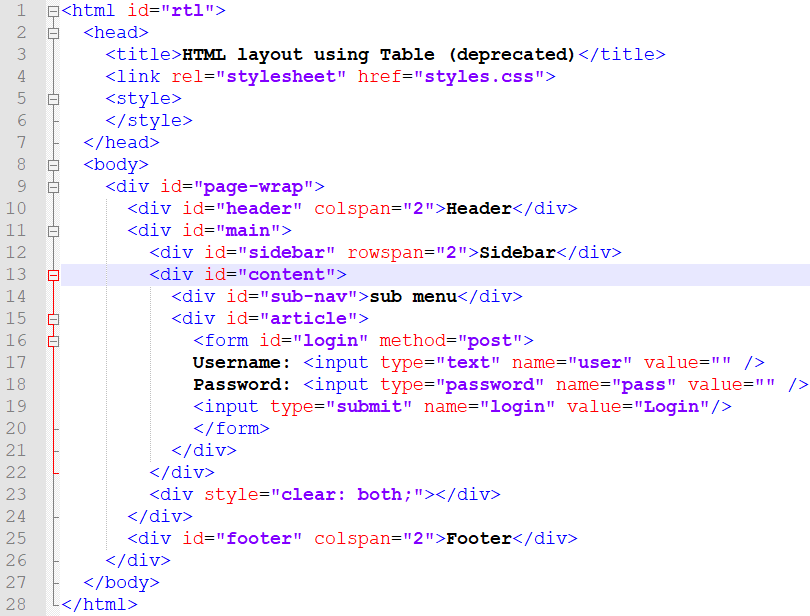
\includegraphics[width=\linewidth]{Images/html}
\caption{نمونه کد \lr{HTML}}
\label{fig:HTML}
\end{figure}

از خواص این نوع تعریف لایه کاربری: تعریف قسمت های مختلف صفحه (دکمه ها، فرم ها، زیرصفحه و ...) در کنار مشخصات و ویژگی های آنها (رنگ، فونت، ...) و حتی کد های رویداد های مختلف در کنار هم است.

{\bf مزایا: }\cite{htmlpros}
\begin{enumerate} 
\item این مدل توصیفی است، یعنی برنامه نویسی بدون نیاز به کد نویسی به توصیف لایه کاربری می پردازد.
\item زبان ساده و خوانا، قابل استفاده برای نا-برنامه نویسان (طراحان، دانش آموزان و ...)
\cite{html4spec}
\item چشم پوشی از خطا: اگر در توصیف لایه کاربری خطایی (در بارگزاری یا حتی سمت برنامه نویس) رخ دهد کل برنامه بی استفاده نمی شود.
\end{enumerate} 

{\bf معایب:}\cite{htmlcons}
\begin{enumerate} 
\item فقط امکان تولید صفحات استاتیک به تنهایی دارد
\item مخلوطی از تمامی منطق برنامه، ظاهر کاربری، کنترل و اطلاعات. باعث عدم امکان توسعه خطی در پروژه های بزرگ و سازمانی می شود.
\item نیازمند دیگر ابزار جهت پویا سازی مثل جاوااسکریپت، activeX و ...
\item صاحب و مدیر StateMachine است و برنامه نویس فقط با event ها از تغییرات وضعیت با خبر می شود. و کنترل کاملی روی آن ندارد. این مسئله باعث به وقوع پیوستن nonDeterministic States می شود.
\end{enumerate} 

\subsection{\lr{WindowsForms, UWP, WPF}}
\label{WindowsForms}
پلتفرم WindowsForms تکنولوژی قدیمی بر بستر WindowsAPI ارایه می شود و به طور کلی ابزاری جهت پیاده سازی رابط کاربری گرافیکی برای برنامه های ویندوزی (GUI) است.
در این پلتفرم جهت توصیف لایه کاربری مستقیما با LayoutEditor نسبت به تعریف رابط کاربری اقدام می کنیم.
ایده پشت این پلتفرم Form-Based بودن است. به این شیوه که تمامی صفحاتی که کاربر با آن تعامل می کند در حقیقت فرمی جهت ورود اطلاعات و دریافت بازخورد از اوست.

\begin{figure}[h!]
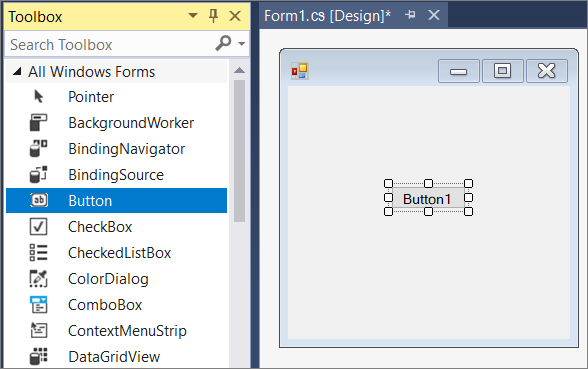
\includegraphics[width=\linewidth]{Images/winform}
\caption{نمونه طراحی با ویرایشگر \lr{WinForm}}
\label{fig:WinForm}
\end{figure}

نسخه بروزتر از این پلتفرم UWP و WPF که به ترتیب برای توسعه برنامه های چند سکویی و دسکتاپ طراحی شده اند دارای زبانی جهت توصیف لایه کاربری به نام XAML هستند.
 این شیوه شباهت بسیاری به ضفحات HTML داشته و بیشتر مزایا و معایب آن در این شیوه هم صادق است.
\cite{winform}


\subsection{\lr{Android}}
\label{Android}
لایه های کاربری در اندروید، به صورت از پیش تعریف شده در فایل XML هایی به عنوان layout برنامه ایجاد می شوند. برنامه نویس امکان ویرایش این فایل را چه به صورت مستقیم و متنی و یا با کمک LayoutEditor اقام به تولید این لایه های کاربری می کند.
در حین اجرای هر Activity (که نمایانگر قسمتی از منطق برنامه) است، این لایه کاربری بارگزاری می شود و نمایش داده می شود.
برای ایجاد هرگونه تغییرات (از جمله افزودن مدیریت رویدادی مثل کلیک) باید ایتدا آن عنصر لایه کاربری را پیدا کرده، رفرنسی از آن را نگه داری و اقدام به اعمال تغییرات مد نظر در آن رفرنس کنیم.\cite{androidlayout}

\begin{figure}[!h]
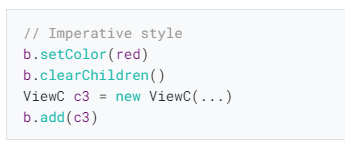
\includegraphics[width=\linewidth]{Images/android}
\caption{نمونه کد برنامه \lr{Android}}
\label{fig:Android}
\end{figure}

لازم به ذکر است که این نگه داری رفرنس در ادامه باعث بروز MemoryLeak ها می شود. این خطا یکی از رایج ترین خطاهای برنامه های اندرویدی است که نیاز به بررسی جداگانه یا توجه مضاعف برنامه نویس جهت مدیریت آنها دارد. 
\cite{androidavoidmemleak}
\cite{androidmemleak}

\begin{figure}[!h]
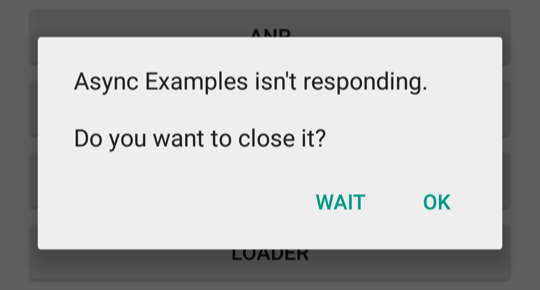
\includegraphics[width=\linewidth]{Images/android-error}
\caption{پیام خطایی آشنا، که MemoryLeak یکی از دلایل بروز آن است}
\label{fig:AndroidError}
\end{figure}

سیستم لایه کاربری اندروید، یکی از معیوب ترین سیستم ها در پلتفرم های با بیشترین استفاده را دارد. یکی از این دلایل قدیمی و متفاوت بودن ورژن های مختلف اندروید روی میلیون ها دستگاه فروخته شده در دهه گذشته است. طراحان جهت سازگاری برنامه های تولید شده با ورژن های قدیمی و همچنین معرفی قابلیت های جدید مجبور به پیاده سازی \lr{Support Library} های مختلف برای قسمت های مختلف محیط کار شدند. به طوری که استفاده از این کتابخانه های پشتیبانی بدون افزودن قابلیتی جدید به برنامه ها در اندروید های بروز به حجم فایل نصبی (APK) برنامه چندین مگابایت می افزودند و حتی مصرف رم و حافظه دستگاه افزایش پیدا میکرد. از طرفی هاستفاده از همین کتابخانه های پشتیبانی در دستگاه های قدیمی تر باعث کاهش سرعت و کارایی و حتی مصرف باتری بیشتر یا داغ کردن دستگاه می شد.
در ادامه با معرفی دسته کتابخانه JetPack گوگل تمرکز خود را برروی ارایه راهکار های خارج از پلتفرم به جای ارایه آنها درون هسته سیستم عامل اقدام کرد.
\cite{androidjetpack}

\begin{figure}[h]
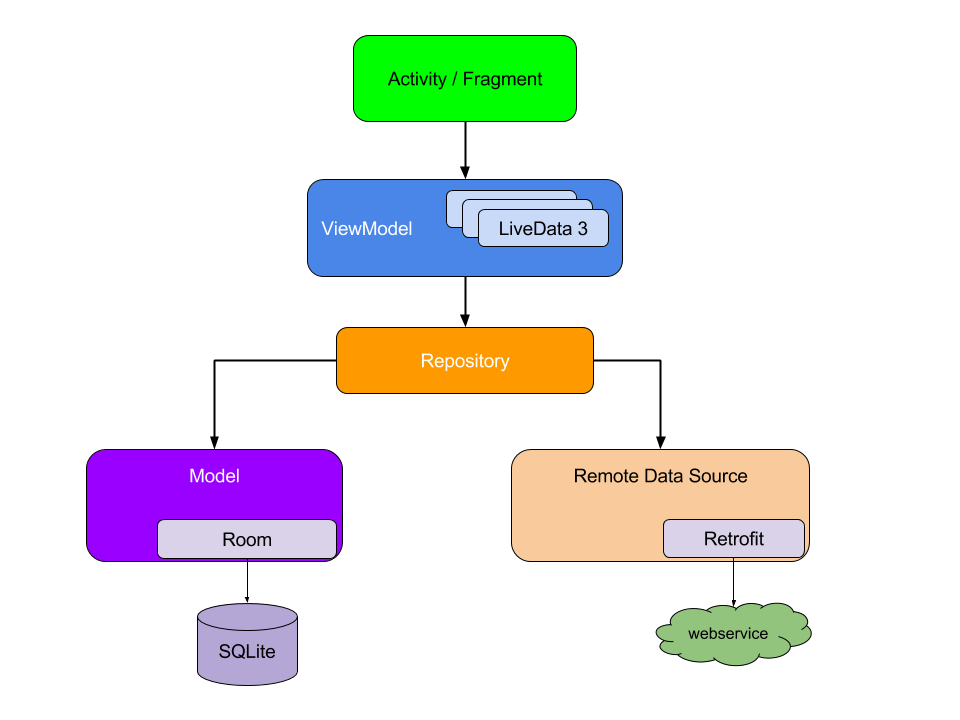
\includegraphics[width=\linewidth]{Images/android-arch}
\caption{شمایی از ساختار جدید ارایه شده گوگل برای برنامه ها}
\label{fig:AndroidArch}
\end{figure}

\section{زمینه}
\label{Context}
تا کنون با تعدادی از شیوه های تولید رابط کاربری قدیمی آشنا شدیم. در اکثر این شیوه ها برنامه نویس هیچ گونه مدیریتی بر وضعیت ماشین (برنامه) و محتوای نمایش داده شده به کاربر به طور مستقیم ندارد. بلکه با استفاده از ویجت های ارایه شده هر پلتفرم و با اتکا به رویداد های گزارش شده آنها به بروزرسانی وضعیت مد نظر می پردازد.

این شیوه از مدیریت وضعیت و اتکا به پلتفرم های گوناگون (با امکان آپدیت و تغییرات) باعث مشکلات بسیاری در برنامه ها می شود.

%\begin{figure}[h!]
%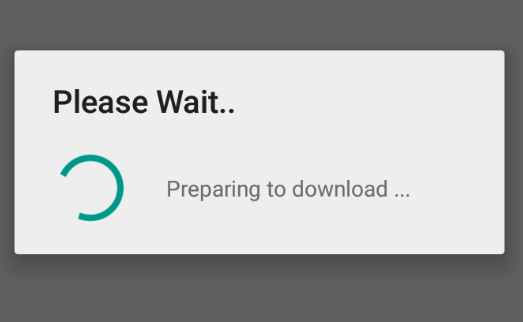
\includegraphics[width=\linewidth]{Images/loading}
%\caption{نمونه دیالوگ درحال بارگذاری قبل از چرخش}
%\label{fig:Loading}
%\end{figure}

اکثر ما تا کنون با برنامه هایی که برخلاف انتظار برنامه نویس به وضعیتی نامطلوب رفته اند (فرضا یک دیالوگ "درحال بارگزاری" در یک برنامه اندرویدی که با چرخش صفحه ناپدید می شود اما از دید برنامه هنوز باید نمایش داده می شد). یکی از مهمترین دلایل این تجارب، نه از عدم آگاهی توسعه دهنده بلکه از {\bf غیر قابل پیش بینی بودن پلتفرم} ایجاد می شود.

جهت مدیریت اینگونه وضعیت های از قبل پیشبینی نشده که اکثرا به علت نقص در پلتفرم، بروز نبودن پلتفرم در دستگاه کاربر (مثل نسخه اندرویدی دستگاه)، عدم شناخت کافی توسعه دهنده از ویژگی ها و عکس العمل های هر کامپوننت در شرایط گوناگون نشات می گیرد، مستلزم به بکارگیری تیم آزمایش محصول و همچنین فرایند پیچیده تر دریافت گزارش های خطا از کاربر می شود. 
حتی گاهی مدیریت یک وضعیت ناخواسته از خود منطق برنامه پیچیدگی بیشتری پیدا میکند.

یکی دیگر از موارد مهم، Reusability کد ها و کامپوننت هایی که یک برنامه نویس تولید و استفاده می کند است. در شیوه سنتی به دلیل وابستگی کامل برنامه نویس به زمینه ای که در آن یک کامپوننت نوشته می شود (از جمله موقعیت قرار گیری در صفحه، المنت های دیگر صفحه و ...) امکان استفاده از یک کامپوننت در دیگر جاهای برنامه کمتر و فرایند آماده سازی یک کامپوننت برای استفاده در پروژه های دیگر خیلی هزینه زیادی دارد.

اکثر مشکلات اشاره شده در این قسمت و قسمت های قبل از عدم کنترل برنامه نویس بر وضعیت کنونی برنامه و همچنین متمرکز نبودن مرجعیت درستی وضعیت در کل برنامه است. 
برای مثال: به این صورت که از دید برنامه نویس چک باکس شماره 1 فعال و چک باکس 2 غیر فعال است. با تغییر این انتخاب توسط کاربر در اکثر پلتفرم ها ابتدا وضعیت تغیر پیدا کرده و سپس تغییر جدید به برنامه نویس از طریق Event ها اطلاع داده می شود. و برنامه نویس کنترلی روی این تغییر ندارد.

\section{راه کار}

راه حل این مسئله فرستادن کل فرایند رسیدیگی و مدیریت وضعیت ها به برنامه نویس و رندرینگ و ... به پلتفرم است.
همچنین کامپوننت های تشکیل دهنده لایه کاربری هیچ گونه وضعیتی آشکار (قابل مدیریت توسط برنامه نویس) نگه داری نکنند. به این ترتیب حتی تغییر وضعیت یک دکمه رادیویی، تایپ در یک تکست باکس هم با اطلاع و موافقت برنامه نویس صورت میگیرد.

برای پیاده سازی این شیوه تولید کامپوننت های لایه کاربری نیاز است که تغییری در نحوه نگاه به لایه های کاربری به طور کلی بیاندازیم. از جمله:

\begin{enumerate} 
\item هر کامپوننت فقط باید به نقش انحصاری خود بپردازد و در کار بقیه قسمت ها تغییری ایجاد نکند.
\item اطلاعات مورد نیاز جهت پیاده سازی به کامپوننت به آن داده می شود. همچنین کامپوننت از هرگونه تغییری در اطلاعات باید آگاه شود.
\item کامپوننت ممکن است جهت اجرای نقش مشخص شده خود، دارای وضعیتی داخلی باشد که البته هیچ تاثیری در وضعیت کلی برنامه نباید بگذارد.
\item کامپوننت ها نباید وابستگی به والد یا فرزندان خود داشته باشند و به تنهایی و در هر محیط و usecase بتوانند وظیفه مربوطه را انجام دهند.
\end{enumerate}

یکی از دیدگاه های مفید در این زمینه به این صورت مطرح می شود که:

\begin{figure}[h!]
\centering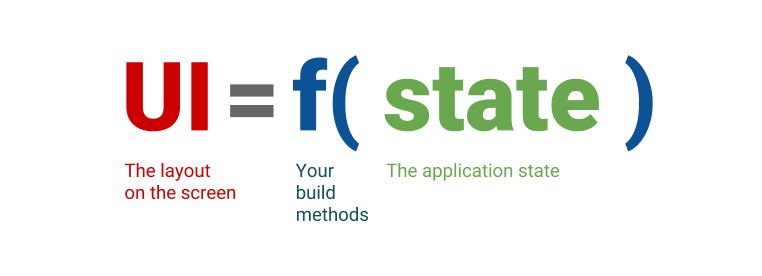
\includegraphics[width=\linewidth]{Images/ui_function}
\caption{\lr{UI is result of application function on state}}
\label{fig:UI_Func}
\end{figure}

به این معنی که هرگونه تغییر در وضعیت برنامه در ظاهر کاربری اثر میگذارد و نه برعکس.
ظاهر کاربری هیچگونه مسیولیتی در زمینه صحت سنجی، بروز رسانی، مدیریت، بارگذاری و پردازش اطلاعات ورودی و خروجی و همچنین وضعیت فعلی برنامه ندارد و تنها مسئولیت آن به نمایش گذاشتن وضعیت فعلی اطلاعات برنامه است.

\section{پلتفرم های امروزی}
در قسمت قبل به برسی راه حل کلی این مدل پیاده سازی آشنا شدیم. حال در ادامه چندین پیاده سازی این راه کار را بررسی می کنیم:

\subsection{\lr{React}}
توسعه دهنده: فیسبوک ، مجوز: MIT. این فریم ورک در اصل یک موتور نمایش اطلاعات در DOM است. به همین علت هرگونه مدیریت وضعیت و ... نیازمند کتابخانه های کمکی جهت مدیریت وضعیت برنامه از جمله Redux نیازمند است.
کامپوننت های تولید شده توسط این فریم ورک به صورت تگ های HTML درون برنامه استفاده می شوند. همچنین تمامی وضغیت مورد نیاز کامپوننت در ابتدای ایجاد آن کامپوننت به آن ارسال می شود.

\begin{figure}[h!]
\centering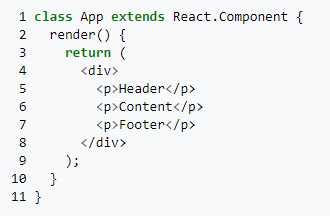
\includegraphics[width=\linewidth]{Images/react}
\caption{\lr{A simple application component in ReactJS}}
\label{fig:React}
\end{figure}

از مزایای سیستم ComponentBased فیسبوک قابلیت جابجایی آن است. اکثر کامپوننت های طراحی شده در پروژه شما بدون نیاز به تغییری قابلیت ایمپورت و استفاده درجا دارند.
این قابلیت از آنجا که تمامی دیتای مورد نیاز و وابسته به کامپوننت حین استفاده از آن تخصیص داده میشود و هیچ گونه وابستگی به دیتا استاتیک یا گلوبال وجود ندارد امکان پذیر شده است. \cite{react}

\begin{figure}[h!]
\centering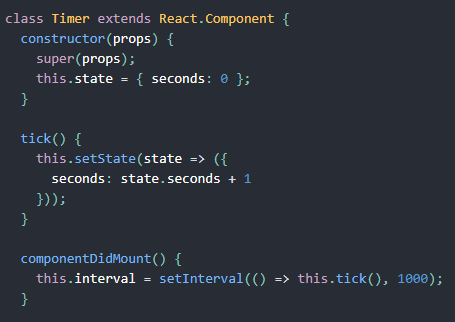
\includegraphics[width=\linewidth]{Images/react-stateful}
\caption{\lr{an Stateful component in React}}
\label{fig:ReactُStateful}
\end{figure}




\subsection{\lr{Flutter}}
توسعه دهنده: گوگل ، مجوز:BSD 3. این فرم ورک جهت تولید لایه های کاربی چند سکویی با هدف کنترل تمام پیکسل های صفحه با ایده گیری از React تولید شد.
زبان این فریم ورک Dart است که شباهت بسیار زیادی به جاوا دارد.

در فلاتر مثل React ما به توصیف لایه های کاربری می پردازیم. همچنین کد منطق نرم افزار می تواند (توصیه نمی شود) در کد لایه کاربری ترکیب شود.
از مزیت این فریم ورک سرعت فوق العاده بالای آن، چند سکویی (اندروید، آی او اس، وب، ویندوز، مک، ...) بوده و امکان کنترل در سطح پیکسل به پیکسل برنامه را به برنامه نویس می دهد.
کامپوننت های نوشته شده در فلاتر به نام ویجدت شناخته می شوند و در دو حالت نوشته می شوند:
حالت Stateless به معنی اینکه ویجدت خود حاوی هیچ گونه وضعیتی نیست و
حالت Stateful به معنای اینکه ویجت برای عملکرد صحیح نیاز به نگداری تعدادی وضعیت داخلی دارد.

\begin{figure}[h!]
\centering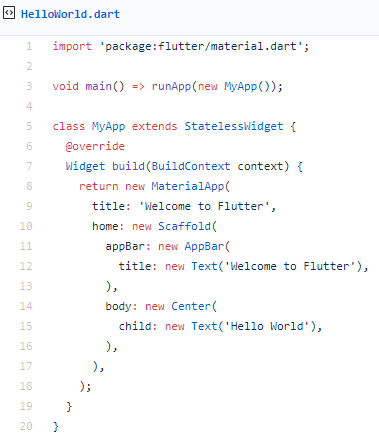
\includegraphics[width=\linewidth]{Images/flutter-code}
\caption{\lr{Simple hello world application in flutter}}
\label{fig:FlutterCode}
\end{figure}

مطابق شکل \ref{fig:FlutterCode} قابل مشاهده است که حتی اپلیکشن تعریف شده در فلاتر به صورت یک ویجت تعریف و مصرف می شود.
این یکسان سازی کاربری در کل پلتفرم باعث سادگی و همگرایی کلی برنامه نویس و طراح می شود.
لازم به ذکر است فلاتر یکی از محبوب ترین فریم ورک های برای نابرنامه-نویسان  و طراحان جهت آشنایی با برنامه نویسی، طراحی و ارایه پروتوتایپ های سریع از برنامه است.

از مزایای دیگر این فریم ورک چند سکویی بودن برنامه و متحد الشکل بودن نتیجه بین همه سکو های اجرای برنامه است. این قابلیت در خطوط تولید برنامه ها در شرکت های استارت آپی با تیم توسعه کوچک و همچنین شرکت ها با برنامه های بزرگ بسیار کاربردی است. به این علت که مدیریت و نگهداری یک Code Base و ارایه قابلیت های جدید و رفع باگ های گزارش شده همزمان صورت می گیرد. شرکت های مختلف پس از مهاجرت به فلاتر اکثرا تجربه ای واحد در بهبود تیم توسعه و افزایش سرعت و بهبود تجربه کاربری داشته اند. \cite{flutter-story}

\begin{figure}[h!]
\centering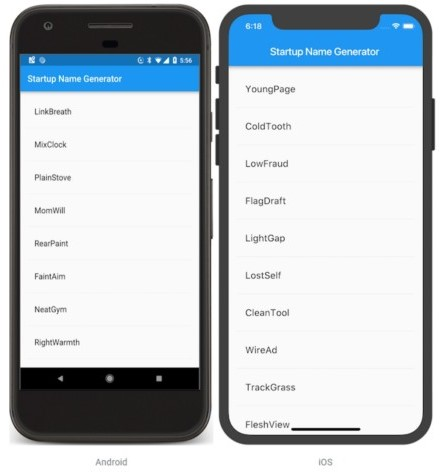
\includegraphics[width=\linewidth]{Images/flutter}
\caption{\lr{a Flutter App run in both android and iOS}}
\label{fig:Flutter}
\end{figure}


\subsection{تازه وارد ها}
پس از معرفی و موفقیت Flutter و React کتابخانه های گوناگونی با همین ایده شکل گرفته اند. از جمله
\href{}{Swift UI}
مختص تولید لایه های کاربری نوین برای macOS، iOS، iPadOS و tvOS یا
\href{}{Android Compose}
ویژه تولید لایه های کاربری جدید اندروید.

این کتابخانه های جدید اکثرا در مرحله پیش نمایش یا بتا هستند و به طور قطعی نمی توان از کارایی و عملکرد آنها اطلاع پیدا کرد، اما می توان این نتیجه را گرفت که: {\bf    بازار آینده تولید روابط کاربری به سمت این ایده حرکت می کند.}

\section{بهبود تجربه}
استفاده از مدل برنامه نویسی جدید علاوه بر مزایا، به دلیل جدید بودن 
شیوه کار با این تکنولوژی ها بعضی سختی هایی هم دارد. 
در اکثر این تکنولوژی ها به توصیف لایه کاربری به همان شیوه ای که در صفحات HTML به صورت درختی تعریف میشدند، می پردازیم.
این شیوه در لایه های کاربری غنی و پر جزئیات بعضی باعث تورفتگی های با درجه زیاد می شود.
راه کار هایی برای این گونه مشکلات ارایه شده از جمله تعریف تابع به تابع قسمت های مختلف و لینک به یکدیگر یا در زبان هایی مثل Swift، Kotlinو جدیدا Dart با تعریف extension function های کاربری این تو رفتگی ها را از دید کاربر محو می کنند.

\begin{figure}[h!]
\centering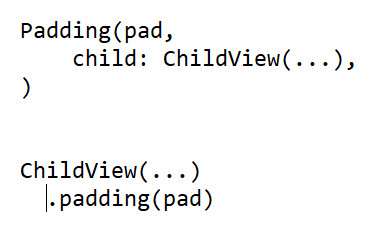
\includegraphics[width=\linewidth]{Images/ext}
\caption{\lr{convertion of hierachy to extension function}}
\label{fig:extension}
\end{figure}


\section{نتیجه گیری}
با فراگیری استفاده از تکنولوژی های جدید فوق، تیم های توسعه دهنده برنامه ها به شکل چشم گیری تغییر شکل پیدا خواهند کرد. روش ها و نگاه ها به فرایند توسعه کاملا عوض شده و در ادامه با افزایش جمعیت جامعه و ابزار های متن باز و ... شاهد تحولی در برنامه های موجود در بازار خواهیم بود.
شایسته است که برنامه نویسان فعال در این حوزه، پیشاپیش نسبت به فراگیری ، تست و کسب تجربه با این تکنولوژی ها آشنا شوند و در آینده بتوانند در رقابت با بازار جهانی سطح بالایی از محصولات نرم افزاری به بازار ارایه دهند.
همچنین گسترش ابزار ها، کامپوننت های فارسی، ترجمه یا همگام سازی موارد فعلی نیز در گسترش این تکنولوژی ها در برنامه های داخلی کمک شایانی می کند.

\bibliography{lib}

%\theendnotes
\end{document}


